\section{LIMS}

 \begin{figure}[h]
 \centering
 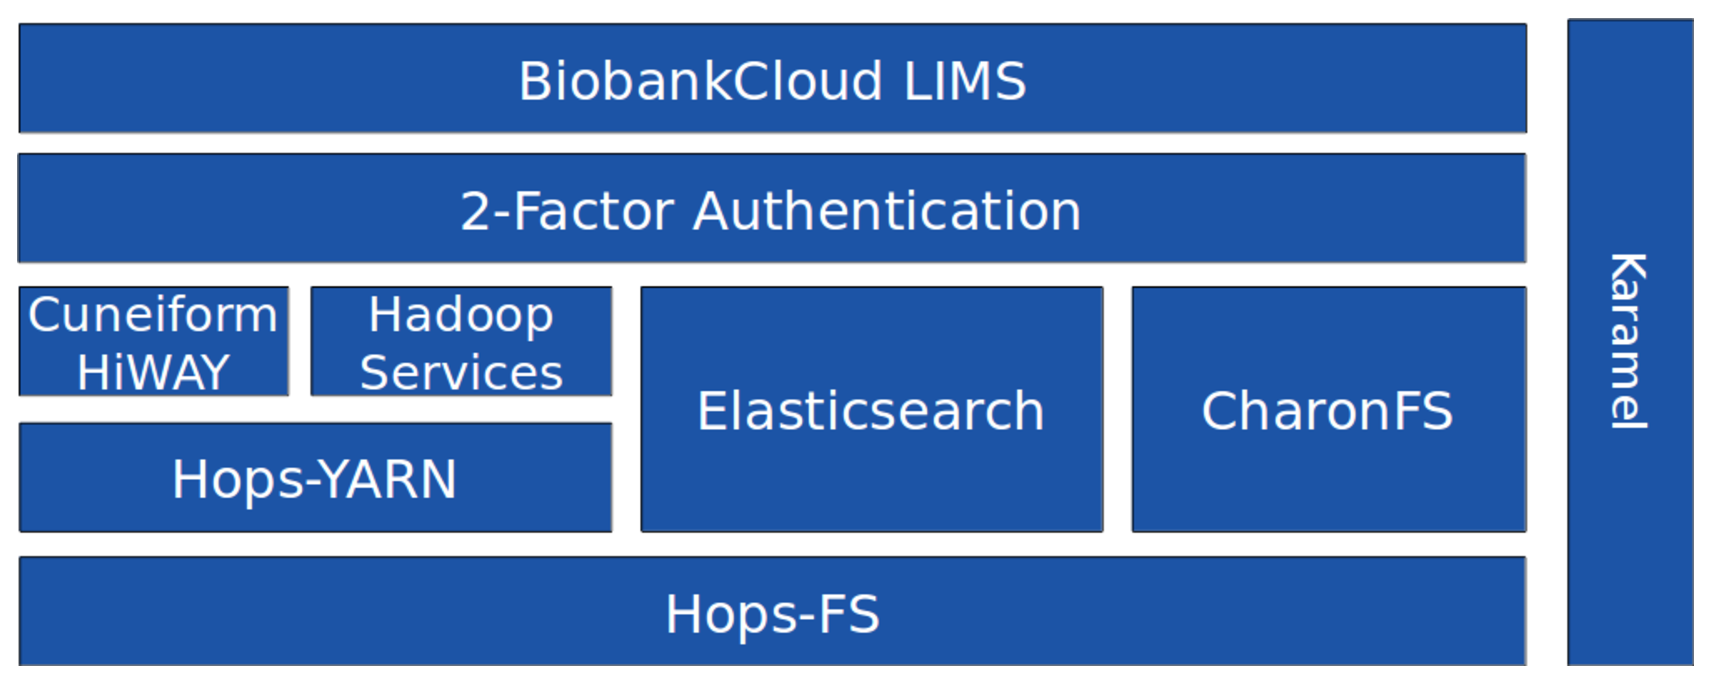
\includegraphics[scale=0.8]{./imgs/stack.eps}
 % stack.eps: 0x0 pixel, 300dpi, 0.00x0.00 cm, bb=0 -1 805 312
 \caption{BiobankCloud Architecture}
 \label{fig:lim}
\end{figure}


In BiobankCloud, we are using our distribution of the Hadoop Filesystem (HDFS), HopsFS, to store large genomic files. HopsFS scales to store 100s of millions of files. There is a need to organize the files in such a manner that they can easily be logically grouped and searched. Typically, such functionality requires metadata for the files and directories, such as filename and last accessed time. For biological samples, much more extensive metadata is required for files that relate to biological samples. We need information such as the sample collection it belongs to, the type of sample, and donor information. BiobankCloud enables Biobankers who are not programmers to design such metadata, link it to samples, and then edit sample metadata using UI support. The metadata is transparently indexed to enable free-text searching for samples, sample collections, and studies. Our solution is based on the industry-standard Elasticsearch platform. Importantly, we guarantee the metadata's integrity by implementing an eventually consistent replication model that asynchronously copies updates to metadata from our distributed database to Elasticsearch. The distributed database uses foreign keys to guarantee the integrity of the metadata and the referrent genomic data. Mutations to the metadata or removal of the sample will mutate or remove the metadata in Elasticsearch within seconds.


Biobankers can use a web application to design new tables that are transparently added to the database and have foreign-key constraints on existing files or directories in the system, thus maintaining the integrity of the metadata. Our system automatically exports metadata to Elasticsearch from where it can be searched using freetext by the user. We support both the automated indexing of files and directories in Elasticsearch as well as custom-designed metadata.

BiobankCloud introduces \textbf{DataSets} as a new abstraction to Hadoop, where a DataSet consists of a related group of directories, files, and extended metadata. DataSets can be indexed and searched and are the basic unit of data management in BiobankCloud; all user-generated files or directories belong to a single DataSet. In Biobanking, a sample collection would be a typical example of a DataSet. 

To allow for access control of users to DataSets, which is not inherent in the DataSet concept, we introduce the notion of \textbf{Studies}. A Study is a grouping of researchers and DataSets with role-based access control where different researchers can be given different access rights to DataSets. The basic user roles we provide reflect the European Data Protection Directive, with a DataOwner (data controller) and a DataScientist (data processer). DataSets can be shared between Studies (when the necessary security, legal, and ethical conditions for sharing are in place).  In BiobankCloud, we use the access control mechanism of HopsFS to implement the Study- and DataSet-based authorization model. 
% Roles are defined and privileges are enforced in HopsFS.